\documentclass[12pt,a4paper]{article} 
\usepackage[portuguese]{babel}
\usepackage[utf8]{inputenc}
\usepackage{amsmath}
\usepackage{graphicx}
\usepackage{booktabs}
\usepackage{float}
\begin{document}
\setcounter{figure}{2}
\setcounter{section}{3}
\setcounter{table}{2}
\setcounter{page}{5}
\section{Relatório}
\subsection{Introdução}
Um retificador é um dispositivo elétrico que converte corrente alternada (\emph{AC}) para corrente contínua (\emph{DC}) que fluí em apenas uma direção. Fisicamente e historicamente, retificadores assumiram várias formas como: Diodos de válvula termiônica, retificadores de óxido de selênio,  retificadores baseados em semicondutores, etc. O objeto de nosso estudo neste experimento, no entanto, serão aqueles construídos a partir de diodos semicondutores.

A necessidade de retificadores surge de aplicações que requerem fontes de correntes \emph{DC}, assim como as que seriam produzidas por uma bateria. Nestas aplicações, também é comum usar um filtro eletrônico, normalmente um capacitor, para que se reduza a pulsação de tensão. A Figura~\ref{fig:esquema_tensao} mostra os blocos típicos que compõem uma fonte de tensão moderna. No entanto, o foco desta prática serão apenas os dois grupos principais de circuitos retificadores, os de meia-onda e os de onda completa.  
\begin{figure}[htpb]
  \centering
  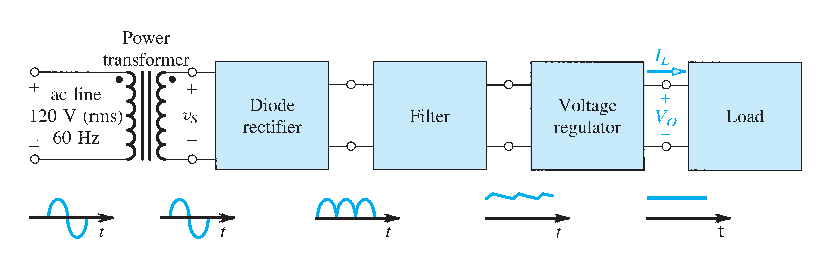
\includegraphics[width=0.8\linewidth]{./blocotransformador.pdf}
  \caption{Diagrama de blocos de uma fonte \emph{DC}.}
  \label{fig:esquema_tensao}
\end{figure}

Os circuitos retificadores de meia-onda , que tem uma implementação possível mostrada pela Figura~1, permitem a passagem de apenas um dos semiciclos de tensão de entrada para a saída. Como a tensão na entrada é alternada, o diodo permite a passagem do sinal, apenas quando estiver diretamente polarizado no semiciclo positivo. Quando estiver no semiciclo negativo, o diodo estará reversamente polarizado e não haverá tensão na saída. A Figura~\ref{fig:meiaonda} nos mostra o output de um circuito retificador de meia onda dado uma entrada senoidal. Neste gráfico, podemos observar que, como um diodo não-ideal tem queda tensão, existe um certo \emph{delay} na curva de output e que o pico do output é reduzido pela queda de tensão do diodo diretamente polarizado ($V_{D}$). Nota-se também que se este sinal é de pouco efeito prático, se for utilizado sem um filtro capacitivo, pois pode ser prejudicial aos componentes eletrônicos. A Figura~\ref{fig:retificadorpico} ilustra o funcionamento de um retificador de pico de meia onda, que nada mais é que um retificador de meia onda com um filtro capacitivo.
\begin{figure}[htpb]
  \centering
  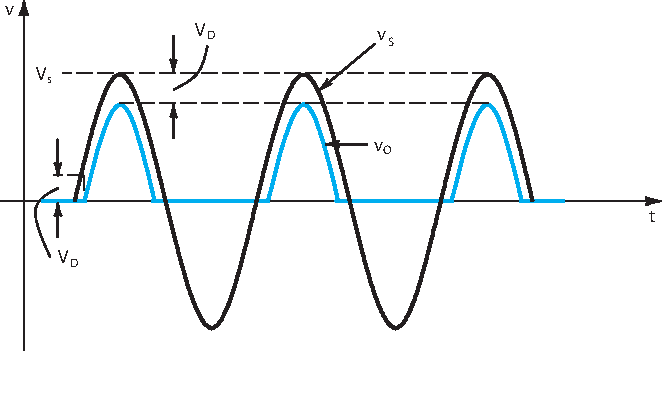
\includegraphics[width=0.8\linewidth]{./meiaonda.pdf}
  \caption{Entrada (preto) e saída (azul) de um circuito retificador de meia-onda. $V_S$ representa tensão de pico da entrada, $V_s$ a tensão de pico da saída, $V_D$ a queda de tensão no diodo diretamente polarizado e $v_o$ o sinal de saída.}
  \label{fig:meiaonda}
\end{figure}
\begin{figure}[htpb]
  \centering
  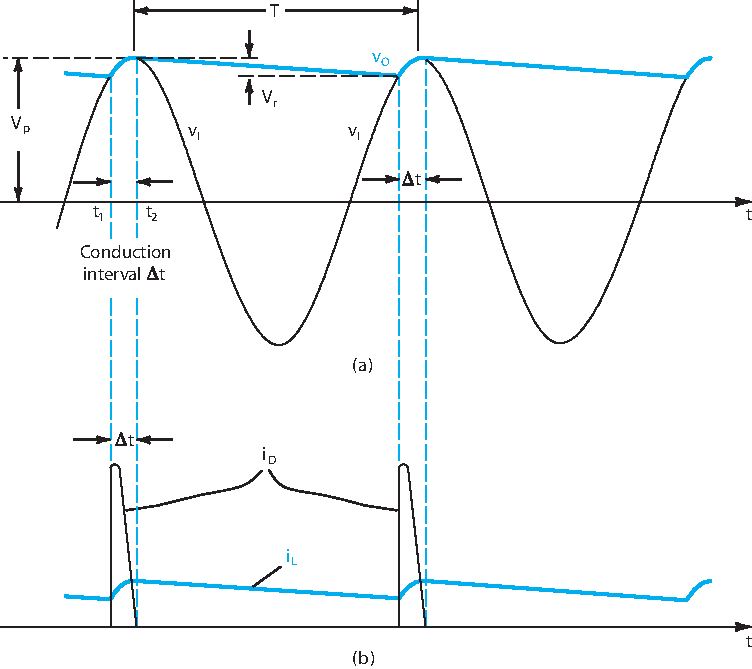
\includegraphics[width=0.7\linewidth]{./retificadorpico.pdf}
  \caption{ \textbf{(a)} Comportamento da tensão de entrada e saída de um filtro capacitor em um retificador de meia onda. \textbf{(b)} Corrente entrega a carga acoplada ao retificado de pico de meia-onda. \textbf{Obs:} Em ambas figuras assumiu-se assumiu-se um diodo ideal.}
  \label{fig:retificadorpico}
\end{figure}

Os circuitos retificadores de onda-completa, que tem uma implementação possível mostrada pela Figura~2, permitem a passagem de sinal por apenas alguns diodos a cada semiciclo positivo, ou negativo, invertendo qualquer sinal negativo para positivo. A Figura~2 é um retificador de onda completa em ponte; quando temos um semiciclo positivo, os diodos $D2$ e $D1$ estarão diretamente polarizados e $D4$ e $D2$ inversamente polarizados o que resultará em um caminho para corrente no ``sentido horário'' e o sinal de entrada pouco mudará, já quando a entrada muda para seu semiciclo negativo, apenas os diodos $D3$ e $D4$ estarão diretamente polarizados, o que resultará em uma inversão do sinal. Podemos analisar estes efeitos com a Figura~\ref{fig:ondacompleta} 

Nota-se que diferentemente do retificador de meia-onda não ``desperdiçamos'' o semiciclo negativo, o que fará com que este circuito tenha uma tensão média de output maior que o anterior. Aqui, também a prática de utilizar um filtro capacitivo é de extrema importância para se aproximar do sinal desejado \emph{DC}, como é ilustrado na Figura~\ref{fig:ondacompletacapacitor}
\begin{figure}[htpb]
  \centering
  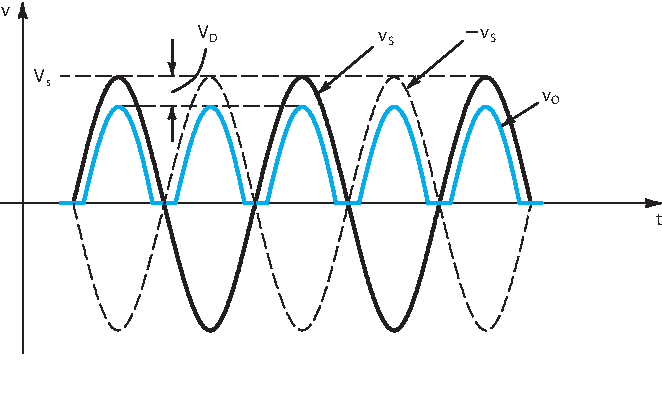
\includegraphics[width=0.8\linewidth]{./ondacompleta.pdf}
  \caption{Entrada (preto) e saída (azul) de um circuito retificador de onda completa. $V_S$ representa tensão de pico da entrada, $V_s$ a tensão de pico da saída, $V_D$ a queda de tensão no(s) diodo(s) diretamente polarizado e $v_o$ o sinal de saída.}
  \label{fig:ondacompleta}
\end{figure}

\begin{figure}[htpb]
  \centering
  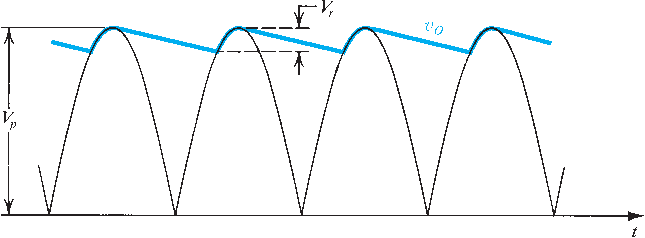
\includegraphics[width=0.8\linewidth]{./ondacompletacapacitor.pdf}
  \caption{Comportamento de um retificador de onda completa com filtro capacitivo, também chamado de retificador de pico de onda completa.}
  \label{fig:ondacompletacapacitor}
\end{figure}
\newpage
\subsection{Análise}
No experimento de número 1 foi montado um retificado de meia onda conforme a Figura~1. Com o auxílio de um osciloscópio verificou-se os seguintes valores:
\begin{align*}
  V_{Avg} =6.353 V\\
  V_{Min} = -0.437 V \\
  V_{Max}= 20.266 V\\
  V_{CA} = 7.873 V
\end{align*}
Ao adicionarmos um capacitor, notamos que os valores se alteraram para:
\begin{align*}
  V_{Avg} =18.995 V\\
  V_{Min} = 17.588 V \\
  V_{Max}= 20.322 V\\
  V_{CA} = 868 mV
\end{align*}
O gráfico da Figura~\ref{fig:221} foi produzido através dos dados obtidos do osciloscópio com o circuito montado como na Figura~1.
\begin{figure}[htpb]
  \centering
  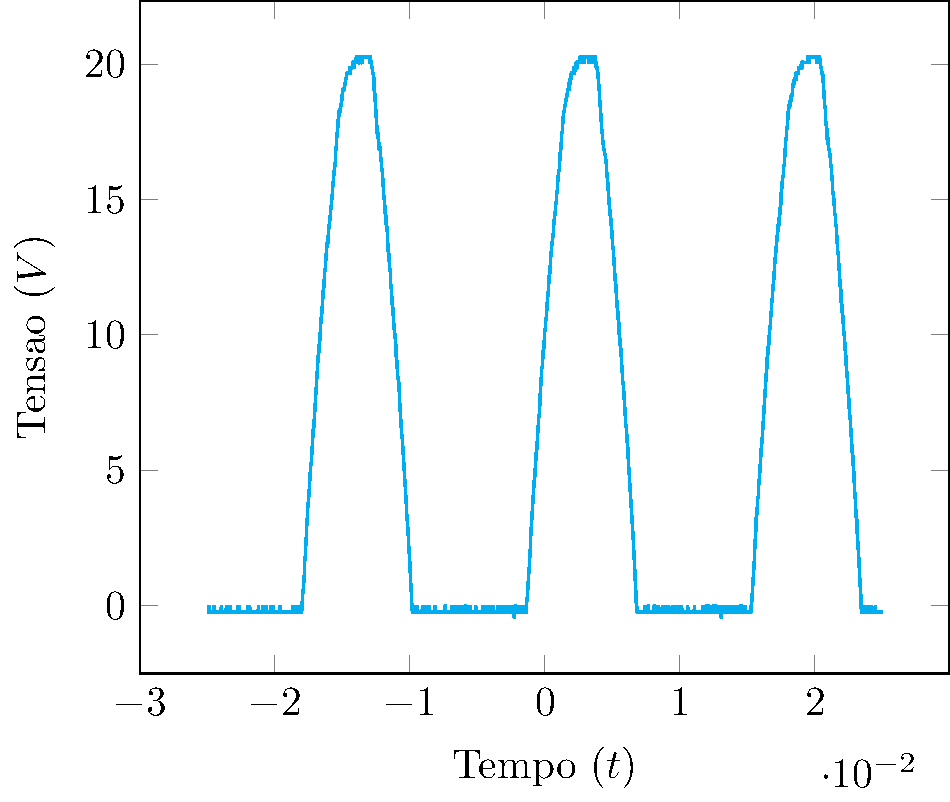
\includegraphics[width=0.8\linewidth]{221.pdf}
  \caption{Sinal de saída do circuito retificador de meia onda sem filtro capacitivo, do experimento de número 1.}
  \label{fig:221}
\end{figure}
Em seguida adicionou-se um capacitor no circuito, o que resultou no gráfico da Figura~\ref{fig:222}. Com os dados das Figuras~\ref{fig:221}-\ref{fig:222}, produzimos a Tabela~1, que nos auxiliou no cálculo do fator de ondulação.
\begin{figure}[htpb]
  \centering
  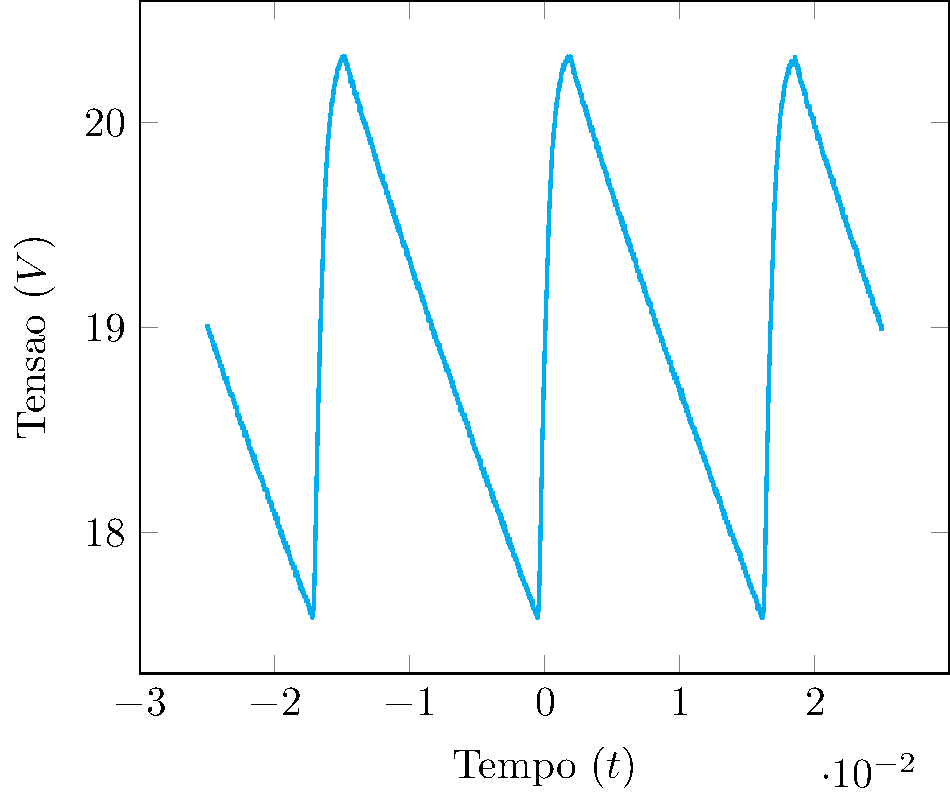
\includegraphics[width=0.8\linewidth]{222.pdf}
  \caption{Sinal de saída do circuito retificador de meia onda com filtro capacitivo, do experimento de número 1.}
  \label{fig:222}
\end{figure}
Para o experimento de número 2, montou-se o circuito descrito pela Figura~2, observou-se o comportamento nos terminais descrito pela Figura~\ref{fig:224}. A entrada do circuito está ilustrada pela Figura~\ref{fig:223}.
\begin{figure}[htpb]
  \centering
  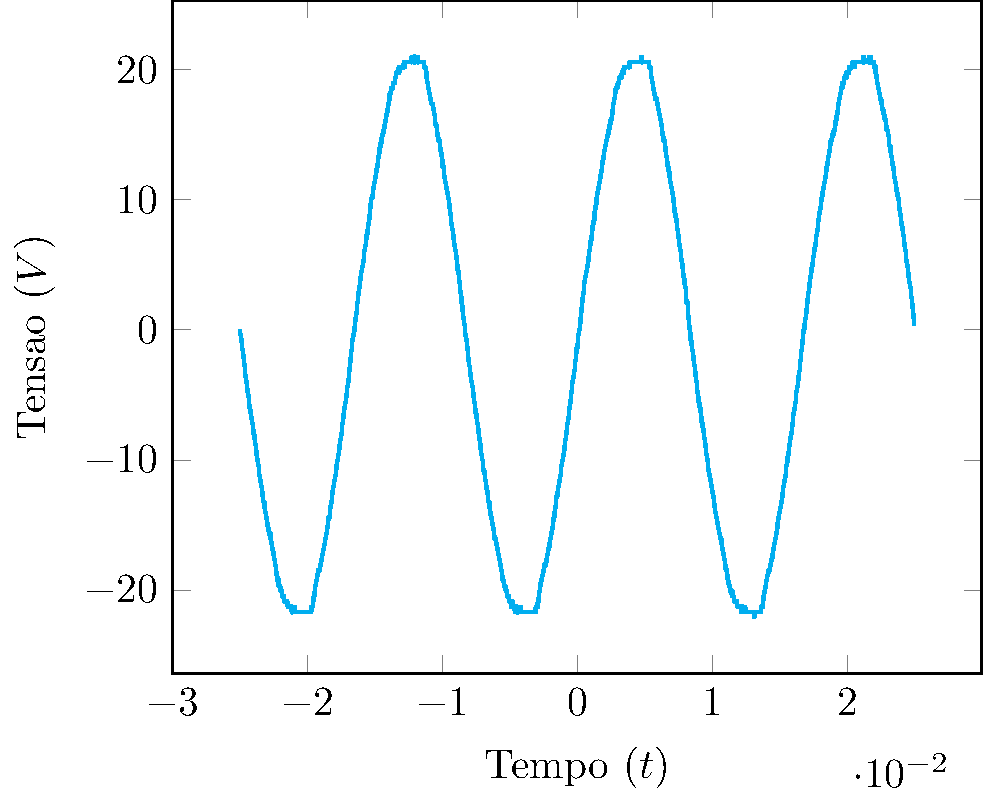
\includegraphics[width=0.8\linewidth]{223.pdf}
  \caption{Sinal de entrada  do circuito retificador de onda completa do experimento de número 2.}
  \label{fig:223}
\end{figure}
\begin{figure}[htpb]
  \centering
  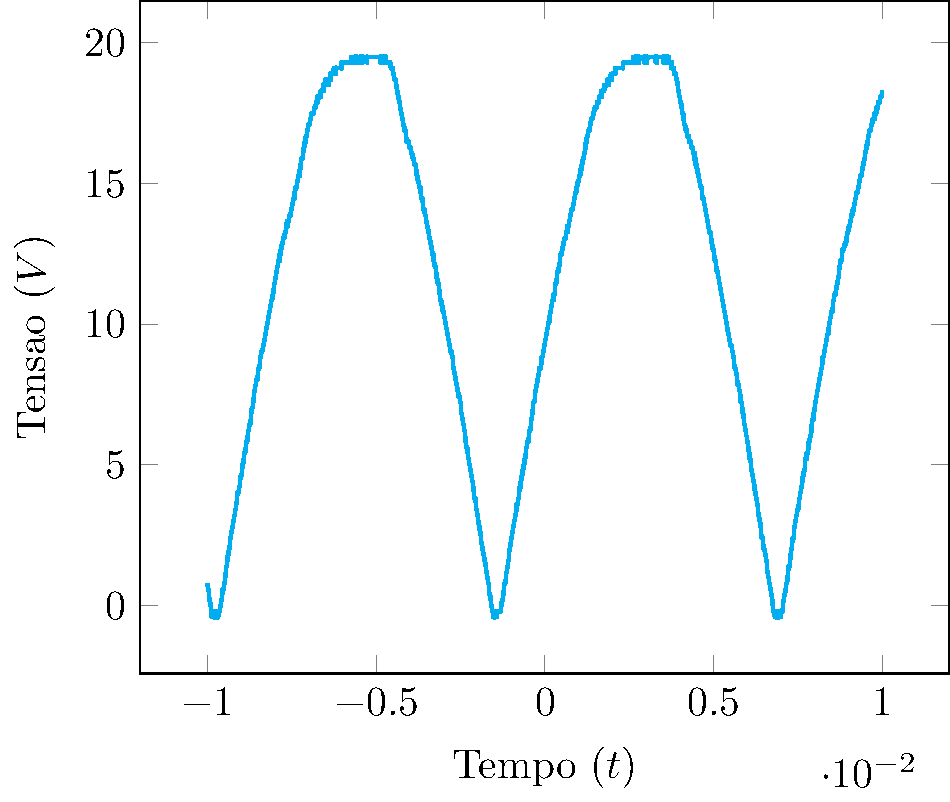
\includegraphics[width=0.8\linewidth]{224.pdf}
  \caption{Sinal de saída do circuito retificador de onda completa sem um filtro capacitivo do experimento de número 2.}
  \label{fig:224}
\end{figure}

Com este mesmo circuito, adicionou-se um capacitor eletrolítico de $100\mu F$. Esta adição mudou o comportamento do sinal de saída, conforme a Figura~\ref{fig:225} nos mostra. Em seguida, o mesmo passo foi repetido, no entanto, com um capacitor de $220\mu F$, o que gerou a Figura~\ref{fig:226}.

\begin{figure}[htpb]
  \centering
  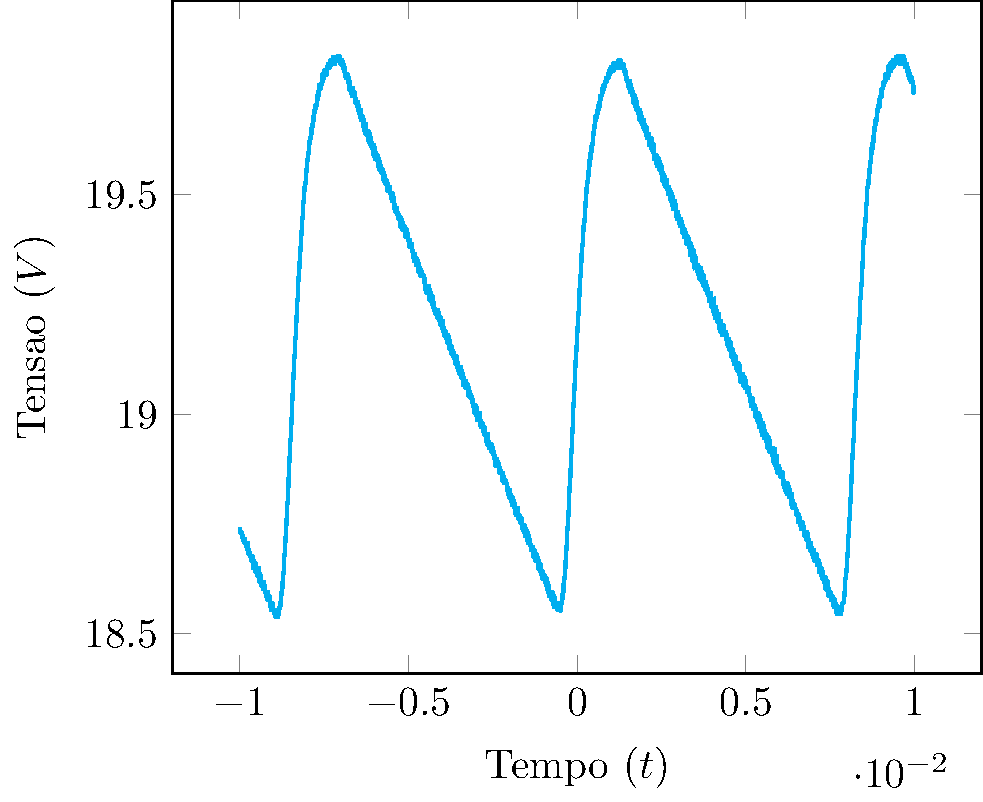
\includegraphics[width=0.8\linewidth]{226.pdf}
  \caption{Sinal de saída do circuito retificador de onda completa com um filtro capacitivo de $100\mu F$ do experimento de número 2.}
  \label{fig:225}
\end{figure}

\begin{figure}[H]
  \centering
  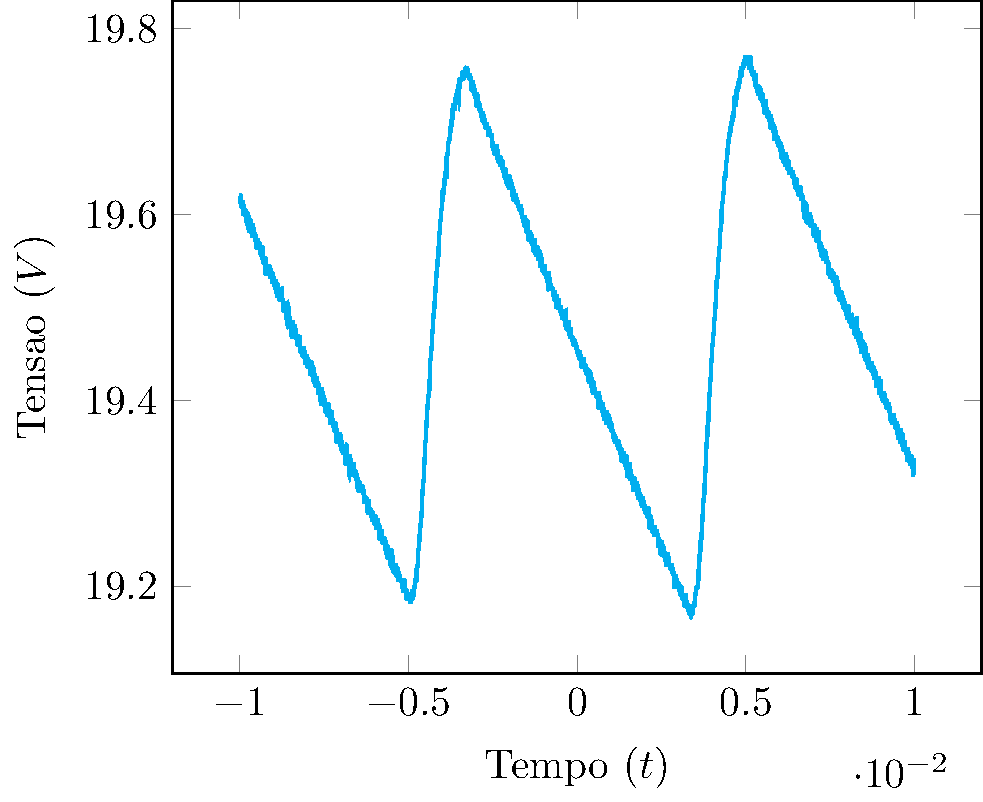
\includegraphics[width=0.8\linewidth]{225.pdf}
  \caption{Sinal de saída do circuito retificador de onda completa com um filtro capacitivo de $200\mu F$ do experimento de número 2.}
  \label{fig:226}
\end{figure}

\newpage
\subsection{Discussões}
Com a ajuda de um osciloscópio, calculou-se o fator de ondulação dos circuitos retificadores com e sem a presença do capacitor. Sabemos que o fator de ripple é dado por:

\begin{align}
            \label{eq:ripple1}
  r=\frac{V_{rms}}{V_{dc}} 
\end{align}
Sendo que $V_{dc}$, para o retificador de meia onda sem filtro capacitivo, é dado por:
\begin{align}
            \label{eq:meiaonda}
   V_{dc}  =0.318 V_{max}  \\ 
\end{align}
E com filtro capacitivo:
\begin{align}
            \label{eq:meiaondacapacitor}
   V_{dc}  \approx V_{max}  
\end{align}
Assim, calculamos os fatores de ondulação:
\begin{align}
  r= \frac{V_{ca} }{0.318 V_{max}}= \frac{7.873}{0.318 \times 20.266}= 1.2216 \\
  r= \frac{V_{ca} }{V_{max}}= \frac{868\times10^{-3}}{20.266}= 0.0428\\
\end{align}
A Tabela~3 sumariza esta nova informação e o fator de onda obtido na Tabela~1. Esperávamos um valor para o fator de ripple do retificador de meia onda sem filtro capacitivo de aproximadamente 121\% ($\frac{0.385V_{max}}{0.315V_{max}}$). Observou-se valores suficientemente próximos a este. 

\begin{table}[htpb]
            \centering
            \caption{Fator de ondulação para as medidas realizadas com o multímetro e com o osciloscópio.}
            \begin{tabular}{c c c c}
              \toprule
              \multicolumn{2}{c }{Multímetro} & \multicolumn{2}{c}{Osciloscópio} \\ \cmidrule(r){1-2} \cmidrule(r){3-4}
            Sem Capacitor   & Com Capacitor  & Sem Capacitor   & Com Capacitor   \\ \cmidrule(r){1-1} \cmidrule(r){2-2} \cmidrule(r){3-3}\cmidrule(r){4-4} 
            123\%        & 4.3\%         & 122.1\%        & 4.28\%          \\ \bottomrule
            \end{tabular}
        \end{table}

        Levando os dados da Tabela~$2$ em consideração, pudemos calcular o fator de ondulação de cada uma das três configurações do circuito.O valor $V_{dc}$, para o retificador de onda completa, foi calculado pela equações abaixo, a equação \ref{eq:ondacompleta} se refere ao circuito sem capacitor, e a equação \ref{eq:ondacompletacapacitor} se refere aos circuitos retificadores de onda completa com filtros capacitivos. O valor do $V_{rms}$ foi obtido através da função do osciloscópio.

 \begin{align}
   \label{eq:ondacompleta}
   V_{dc}  =0.636 V_{max}  \\
   \label{eq:ondacompletacapacitor}
   V_{dc} \approx V_{max}
 \end{align}
\begin{align}
  r_1 = \frac{V_{rms}}{V_{dc}}= \frac{6.5 V}{19.7 \times 0.636 V}= 51.87\%\\
  r_2= \frac{V_{rms}}{V_{dc}} \approx \frac{V_{rms}}{V_{max}} = \frac{411 mV}{19.815}= 2.07 \% \\
  r_2= \frac{V_{rms}}{V_{dc}} \approx \frac{V_{rms}}{V_{max}} = \frac{164 mV}{19.79}= 0.828 \%
\end{align}
O resultado é descrito na Tabela 4. Esperávamos valores de $r$ próximos a $48.7\%$ ($\frac{0.308 V_{max}}{0.636 V_{max}}$) para o retificador de meia onda sem capacitor. Considerando o fator de ondulação como indicativo de qualidade, conclui-se que o retificador de meia onda é melhor com a presença de um filtro capacitivo, pois ambos valores foram significativamente menores que o valor sem filtro capacitivo. Da mesma forma, temos o indicativo que capacitores maiores tendem a nos dar fatores de ondulação melhores. Suspeita que sera confirmado no próximo experimento. 
    \begin{table}[htpb]
        \centering
        \caption{Fator de ondulação para o circuito retificador de onda completa.}
        \begin{tabular}{l c c c}
        \toprule
        & Sem capacitor & Capacitor $100 \mu F$ & Capacitor $220 \mu F$ \\ \midrule
        \multicolumn{1}{c}{Fator de ondulação} & 51.87\%       &  2.07\%  &  0.828\%                \\ \bottomrule
        \end{tabular}
        \end{table}

        Assim, como desejamos um sinal com baixo fator de ondulação, pode-se concluir que o circuito que melhor desempenha é o com capacitor de $220 \mu F$. Isto pode ser verificado com os gráficos gerados a partir dos dados obtidos no osciloscópio; quando observamos a Figura~\ref{fig:224}, notamos uma excursão do sinal de $0$ a $20V$, como desejamos um sinal $DC$ adicionou-se o capacitor de $110 \mu F$, e observou-se na Figura~\ref{fig:225} uma excursão de $1V$ entre $18.5 V$ e $19.5 V$, o que já se parece com um sinal $DC$. No entanto, ao aumentarmos a capacitância do capacitor no circuito para $220 \mu F$ observou-se uma excursão de apenas $0.4 V$, entre $19.2 V$ e $19.6V$, o que rendeu um sinal $DC$ melhor, conforme foi confirmado pelo fator de ondulação da Tabela~4. \\
        O efeito do capacitor foi, em outras palavras, diminuir de forma significativa o efeito de ondulação, já que o sinal excursionou menos e ficou mais constante, assim como desejamos que uma fonte $DC$ se comporte. Capacitores maiores tendem a diminuir a excursão e consequentemente o ripple no sistema é menor.

Nota-se também, pela equação \ref{eq:ripple2}, o relacionamento entre o resistor e o fator de ondulação. Quando a resistência da carga é diminuída, o fator de ondulação tende a aumentar. 
        \begin{align}
            \centering
            \label{eq:ripple2}
            r = \frac{2.4}{R_L C}\times 100\%
        \end{align}        
\newpage
\subsection{Conclusão} 
Esta prática possibilitou um estudo profundo a cerca de retificadores de tensão. Através de diodos e resistores somente, aprendemos configurações padrões para montar estes tipos de circuitos e muito a respeito do funcionamento esperado destes.

Na primeira prática, estudamos o comportamento de um circuito retificador de meia onda e como a inclusão de um capacitor tem um impacto positivo em diminuir o ripple total do circuito.

Estendendo a ideia anterior, o segundo experimento nos mostrou como podemos, a custo de mais complexidade no circuito, ter uma tensão média maior, retificando a onda tanto no seu semiciclo positivo e negativo, com o retificador de onda completa. Estudou-se também o impacto da variação da capacitância do filtro capacitivo no retificador, e conclui-se que altas capacitâncias ajudam na performance do retificador.

Em uma breve comparação entre os circuitos retificadores, estudou-se um parâmetro, o fator de ondulação ($r$), que nos ajudou a avaliar a performance de cada retificador. Finalmente,   conclui-se que o circuito com maior performance foi o circuito retificador de onda completa com filtro de maior capacitância.

\end{document}
